\chapter{Markovin ketju Monte Carlo menetelmät}

Tässä luvussa aiomme esitellä MCMC-metodeja. Esittelemme alaluvussa \ref{gibbs} Gibbsin otanta-algoritmina tunnetun MCMC-menetelmän, ja sitten alaluvussa \ref{Metropolis--Hastings algoritmi} esittelemme Metropolis--Hastings algoritmin. Osoitamme myös, että todellisuudessa alaluvun \ref{gibbs} algoritmi onkin todella vain erikoistapaus luvun \ref{Metropolis--Hastings algoritmi} algoritmista. Pohditaan kuitenkin ensin menetelmän motivaatiota. \cite[s.~94]{koistinen_computational_2009} \cite[s.~269]{monte_carlo_book}
 
\begin{maar}
	MCMC-menetelmiksi kutsutaan jakaumaa $p$ simuloivia menetelmiä, jotka perustuvat siihen, että luodaan ergodinen Markovin ketju $(X_n)$, jolla on tasapainojakaumana jakauma $p$.
\end{maar}

Ketjun ergodisuus takaa siis sen, että ketju konvergoituu jokaisesta tila-avaruuden pisteestä. Se takaa, että ketjun empiirinen keskiarvo
\begin{equation}
	\mathfrak{J}_n = \frac{1}{n} \sum_{t=1}^{n} h(X_t)
\end{equation}
konvergoituu odotusarvoon, eli
\begin{equation}
	\lim_{n\to\infty} \mathfrak J_n \to \mathbb{E}_p[h(X_t)] = \int h(x)p(x)dx
\end{equation}
Tällöin ketjun tiloja voidaan siis käsitellä i.i.d. otoksena tasapainojakaumasta.

Markovin ketjuille (ja useimmille MCMC-menetelmien tuottamille Markovin ketjuille) pätee myös keskeinen raja-arvolause \eqref{CLT}.

\begin{equation}\label{CLT}
	\sqrt{n}\qty(\mathfrak{J}_n-\mathbb{E}_p[h(X_t)]) \to N(0, \sigma^2_h) \qq{kun} n\to\infty
\end{equation}
jossa 
\begin{equation}
	\sigma^2_h = \text{var}_p(h(X_0))+2\sum_{t=1}^{\infty}\text{cov}_p(h(X_0),h(X_t))
\end{equation}

Menetelmän ydin on siis rakentaa systemaattisella tavalla Markovin ketju, jonka tasapainojakaumana on haluamamme simuloitava jakauma. Tämän voisi kuvitella olevan kovin vaikeaa, mutta yllättävästi se onkin melko helppoa.

\section{Gibbsin otanta-algoritmi}\label{gibbs}

\textit{Gibbsin otanta-algoritmi} on tapa simuloida bayesiläistä moniulotteista posteriorijakaumaa (eli ulottuvuuksia vähintään 2), kun suora otanta on hankalaa. Algoritmi on nimetty amerikkalaisen fyysikon, \textit{Josiah Willard Gibbsin} (1839-1903) mukaan, mutta sen todellinen kehittäjä on veljekset \textit{Donald Geman} (1943-) ja \textit{Stuart Geman} (1949-) vuonna 1984 artikkelissa \textit{Stochastic Relaxation, Gibbs Distributions, and the Bayesian Restoration of Images}. 

Aloitetaan määrittelemällä algoritmi. \cite[s.276-277]{gelman_andrew_bayesian_nodate}

\begin{maar}\label{gibbs}
	Olkoot $\theta$ parametrivektori, joka jaetaan $d$:hen osaan tai osavektoriin, eli $\theta = (\theta_1, \theta_2,...,\theta_d)$. Gibbsin otanta-algoritmi määritellään seuraavanlaisesti:
	\begin{enumerate}
		\item Arvotaan permutaatio parametrivektorille $\theta$
		\item Arvotaan uusi tila jokaiselle osavektorille $\theta_j$ ehdollistamalla se jokaiselle muulle parametrille, eli vedetään arvot $\theta_1, \theta_2,...,\theta_d$ jakaumista
		\begin{equation}\label{mcmc:gibbs:maar:2}
			p(\theta_j|\tnm_{-j},y)
		\end{equation}
		arvotun permutaation parametrijärjestyksessä
		\item toistetaan 1-3
	\end{enumerate}
\end{maar}

\begin{huom}
	Jakaumassa \eqref{mcmc:gibbs:maar:2} merkintä $\tnm_{-j}$ viittaa kaikkiin muihin parametrin $\theta$ komponentteihin paitsi $j.$ komponenttiin, näiden tämänhetkisillä arvoilla eli 
		\begin{equation*}
			\tnm_{-j} = (\tn_{1},...,\tn_{j-1},\tnm_{j+1},...,\tnm_{d})
		\end{equation*}
\end{huom}

Yleensä määritelmässä \ref{gibbs} kohdassa 1. ei arvota uutta permutaatiota, vaan permutaatio päätetään alussa, ja sitä pidetään kaikkien algortimin iteraatioiden ajan samana. Tätä kutsutaan \emph{systemaattiseksi Gibbsin otanta-algoritmiksi} (\textit{systematic scan Gibbs sampler}).

\begin{lause}\label{gibbs-proof}
	Määritelmän \ref{gibbs} mukaisen algoritmin tuottama Markovin ketju on jaksoton, pelkistymätön ja Harris palautuva ja sillä on sitten yksikäsitteinen tasapainojakauma $p(\theta)$. \cite{koistinen_computational_2009}
\end{lause}

\begin{proof}
	Voitaisiin osoittaa, että määritelmän \ref{gibbs} algoritmin tuottama Markovin ketju on ergodinen, ja täten konvergoituu tasapainojakaumaan. Ohitetaan se tässä, sillä todistus on melko tekninen.
	
	Olkoot $\tnm$ parametrin alkuperäinen tila, ja $\tn_j$ uusi $j$:nnen parametrin tila. Nyt $\tnm$ ja $\tn_j$ yhteistiheysfunktio on kertolaskusäännöllä.
	\begin{equation}
		p(\tnm)p_j(\tn_j|\tnm_{-j})
	\end{equation}
	Nyt voidaan integroida
	\begin{equation}
		\begin{split}
			\int p(\tnm)p_j(\tn_j|\tnm_{-j}) d\tnm_j &= \int p(\tnm_j|\tnm_{-j})p(\tnm_{-j})p_j(\tn_j|\tnm_{-j}) d\tnm_j \\
			&= p(\tnm_{-j})p_j(\tn_j|\tnm_{-j}) \int p(\tnm_j|\tnm_{-j}) d\tnm_j \\
			&= p(\tnm_{-j})p_j(\tn_j|\tnm_{-j}) \\
			&= p(\tn_j,\tnm_{-j})
		\end{split}
	\end{equation}
	Eli Gibbs otanta-algoritmin päivitys ei muuta jakaumaa. Nyt voidaan soveltaa lausetta \ref{cyclic-kernel-jatkuva}, jolloin voidaan todeta, että koska $p$ tasapainojakauma jokaiselle $p_j(\tn_j|\tnm_{-j})$, niin se on tasapainojakauma niiden yhteis siirtymätiheydelle
	\begin{equation}
		T = \prod_{j=1}^{d} p_j(\tn_j|\tnm_{-j})
	\end{equation}

\end{proof}

Ohitetaan Gibbsin otanta-algoritmin kohdalla toistaiseksi esimerkit, ja palataan siihen kappaleessa \ref{esimerkki}, jossa tarkastelemme laajempaa esimerkkiä lineaarisen regression parissa. Toteutamme tämän Gibbsin otanta-algoritmina.

Gibbsin otanta-algoritmin vaatimus ehdollisista jakaumista voi vaikuttaa jokseenkin rajoittavalta, sillä joskus voidaan tutkia mallia, jolle on vaikea laskea ehdolliset jakaumat. Toisaalta taas joskus saatamme haluta simuloida yksiulotteista jakaumaa Gibbsin otanta-algoritmilla, mutta tämä ei suoraan ole mahdollista sillä algoritmi tarvitsee vähintään kaksiulotteisen parametrin. Tällöin voidaan kuitenkin pienin muunnoksin hyödyntää Gibbsin otanta-algoritmia hyödyntämällä seuraavaa määritelmää \ref{completion}. \cite[s.~374]{monte_carlo_book} 

\begin{maar}\label{completion}
	Olkoot $p$ tiheysfunktio. Tiheysfunktiota $\lambda$, joka täyttää ehdon
	\begin{equation}
		\int_Z \lambda(x,z) dz = p(x)
	\end{equation}
	kutsutaan $p$:n täydellistymäksi (\textit{completion}).
\end{maar}

Tiheys $\lambda$ valitaan siten, että sille voi ratkaista ehdolliset jakaumat. Nyt Gibsin otanta-algoritmi voidaan toteuttaa käyttämällä jakaumaa $\lambda$ ja sen ehdollisia jakaumia. Lauseen \ref{gibbs-proof} tulos pätee myös tässä tapauksessa. Tällöin malliin tulee toki uusi parametri $z$, joka on täysin turha mallin kannalta, mutta avustaa simuloinnissa.


%%%%%%%%%%%%%%%%%%%%%%%%%
%% Metropolis-Hastings %%
%%%%%%%%%%%%%%%%%%%%%%%%%

\section{Metropolis--Hastings algoritmi}\label{Metropolis--Hastings algoritmi}

\textit{Metropolis--Hastings} algoritmi on kehittelijöidenssä \textit{Nicholas Metropolin} (1915-1999) ja \textit{Wilfred Keith Hastingsin} (1930-2016) mukaan nimetty MCMC-menetelmä, jolla voidaan simuloida bayesiläisessä analyysissa käytettäviä posteriori jakaumia myös silloin kun tiheys on mahdotonta määrittää analyyttisesti.

Algoritmin pohjan kehittivät \textit{Stanislav Ulam} ja Metropolis työskennellessään \textit{Los Alamosissa} ja myöhemmin Metropolis kehitteli nykyään \textit{Metropolis-algoritmina} tunnettua algoritmiä ja esittelivät sen artikkelissa \textit{Equation of state calculations by fast computing machines}\cite{metropolis_nicholas_equation_1953}. Tämä versio algoritmista vaati, että pian esiteltävä \textit{ehdotusjakauma} on symmetrinen. Myöhemmin \textit{Hastings} laajenti algoritmin koskemaan myös epäsymmetrisiä ehdotusjakaumia artikkelissa \textit{Monte Carlo Sampling Methods Using Markov Chains and Their Applications}. Esitämme jälkimmäisen version algoritmista, sillä edellinen seuraa jälkimmäisestä suoraan.

\begin{merk}
	TN-jakauma $J_n(\cdot|\cdot)$ on niin sanottu \textit{ehdotusjakauma} (\textit{proposal distribution, jumping distribution}), josta \textit{MH-algoritmissa} arvotaan ehdotustila.
\end{merk}

Nyt kun ehdotusjakauma on määritelty, voidaan määritellä Metropolis-Hastingsin algoritmi seuraavanlaisesti \cite[s.278-279]{gelman_andrew_bayesian_nodate}

\begin{maar}\label{mh-maar}
	Metropolis--Hastings algoritmi on seuraavanlainen
	\begin{enumerate}
		\item Valitaan aloitustila $\theta_0$ tilajoukosta (tämän askeleen aika on $n = 0$)
		\item Generoidaan kandidaatti tila $\theta'$ satunnaisesti ehdotusjakaumasta $J_n(\theta'|\tnm)$
		\item Lasketaan suhde
		\begin{displaymath}
			r = \frac{p(\theta'|y)/J_n(\theta'|\tnm)}{p(\tnm|y)/J_n(\tnm|\theta')}
		\end{displaymath}
		\item Asetetaan
		\begin{displaymath}
			\tn= 
			\begin{cases}
				\theta', \text{todennäköisyydellä} \hspace{0.3cm} \min(r,1) \\
				\tnm, \text{muuten}
			\end{cases}
		\end{displaymath}
		\item Toistetaan 2-5
	\end{enumerate}
\end{maar}

\begin{lause}
	Määritelmän \ref{mh-maar} algoritmi tuottaa Markovin ketjun jolla on uniikki tasapainojakauma $p(\theta)$ 
\end{lause}

\begin{proof}

Todistus nojautuu Markovin ketjun kääntyvyysominaisuuteen (\ref{kaant-disk}) ja (\ref{kaant-jatk}), eli
	\begin{equation}\label{kaant-mcmc}
		T(\tn|\tnm)p(\tnm) = T(\tnm|\tn)p(\tn)
	\end{equation}
	joka on siis riittävä ehto tasapainojakauman olemassaololle. Mietitään kahta tapausta: (1) $\tn \neq \tnm$ ja (2) $\tn = \tnm$.
	Tapauksen (2) siirtymä voi tapahtua kahdella tavalla. Joko kohdassa 4. ehdotus $\theta'$ hylätään, tai se hyväksytään, mutta osutaan sattumanvaraisesti takaisin samaan kohtaan. Kuitenkin selvästi nähdään, että ehto \ref{kaant-mcmc} pätee tilanteessa (2).
	
	Tilanteessa (1) siirtymätodennäköisyys pisteestä $\tnm$ pisteeseen $\tn$ on
	\begin{equation}
		T(\tn|\tnm) = J_n(\tn|\tnm)
		\min\Big( \frac{p(\tn)J_n(\tnm|\tn)}{p(\tnm)J_n(\tn|\tnm)},1 \Big)
	\end{equation}
	Jota voidaan muokata helposti muotoon
	\begin{equation}\label{metr-has-proof1}
		\begin{split}
			T(\tn|\tnm) &= J_n(\tn|\tnm)
		\min\Big( \frac{p(\tn)J_n(\tnm|\tn)}{p(\tnm)J_n(\tn|\tnm)},1 \Big) \\
		&= \frac{1}{p(\tnm)} \min \Big( p(\tn)J_n(\tnm|\tn) , p(\tnm)J_n(\tn|\tnm)  \Big)
		\end{split}
	\end{equation}
	Toistamalla ylläoleva siirtymätodennäköisyydelle pisteestä $\tn$ pisteeseen $\tnm$ havaitaan, että 
	\begin{equation}\label{symmetric}
		T(\tnm|\tn)=\frac{1}{p(\tn)} \min \Big( p(\tnm)J_n(\tn|\tnm) , p(\tn)J_n(\tnm|\tn)  \Big)
	\end{equation}
	lauseke on symmetrinen. Kerrotaan yhtälö \eqref{metr-has-proof1} termillä $p(\tnm)$ ja hyödynnetään ominaisuutta \eqref{symmetric}, jolloin
	\begin{equation*}
	\begin{split}
		T(\tn|\tnm)p(\tnm) &= \frac{1}{p(\tnm)} \min \Big( p(\tn)J_n(\tnm|\tn) , p(\tnm)J_n(\tn|\tnm)  \Big) p(\tnm) \\
		&= \frac{1}{p(\tn)} \min \Big( p(\tnm)J_n(\tn|\tnm) , p(\tn)J_n(\tnm|\tn)  \Big) p(\tn) \\
		&= T(\tnm|\tn)p(\tn)
	\end{split}
	\end{equation*}
	Eli myös tapauksessa (1) yhtälö \eqref{kaant-mcmc} pätee.
\end{proof}

\begin{esim}\label{mh-esim1}
	Ajatellaan kuvitteellista tapausta, jossa meillä jatkuva kaksiulotteinen todennäköisyysjakauma, jonka tiheysfunktio on 
	\begin{equation}
		p(\theta) \varpropto \exp(-5 |\theta_1^2+\theta_2^2-1|)
	\end{equation}
	joka muodostaa regasmaisen 2-ulotteisen jakauman. Valitaan ehdotusjakaumaksi $J_n(\tn|\tnm)$ 2d-multinormaalijakauma 
	\begin{equation}
		J_n(\tn|\tnm) \sim N(\tnm, \sigma^2 I_2)
	\end{equation}
	jossa $I_2$ on $2 \times 2$ yksikkömatriisi ja olkoot $\sigma^2 = 0.01$. Nyt Metropolis-Hastingsin algoritmin avulla voidaan simuloida jakaumaa $p(\theta)$ algoritmilla \ref{mh-maar}. Simuloidaan kaksi Markovin ketjua asettemalla aloitustiloiksi $(0,0)$ ja $(5,5)$, 
	\begin{figure}[h!]
		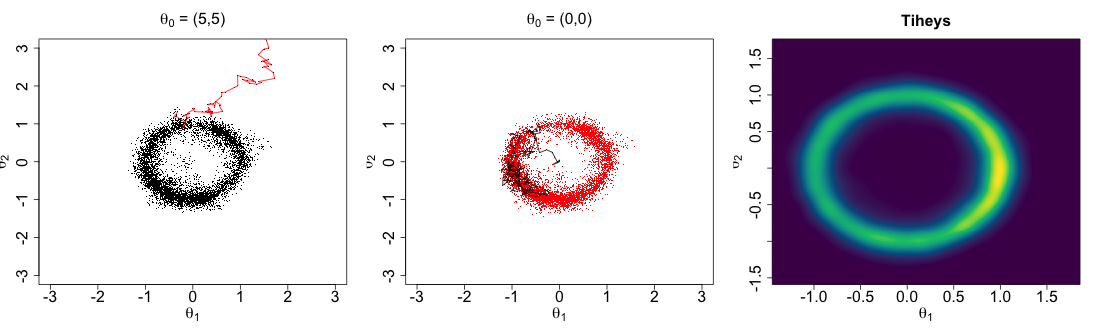
\includegraphics[width=\textwidth]{mhexample1}
		\caption[Kaksiulotteinen Metropolis--Hastings esimerkki]{\textit{Vasemmalla: (5,5). Keskellä: (0,0) Oikealla: tiheysestimaatti (huomaa eri skaala).}}
		\label{kuva1}
	\end{figure}
	kummastakin 10 000 tilaa. Simuloimme myös 200 000 pistettä aloitusarvolla (0,0), joista luodaan tiheysestimaatti. Tulokset löytyy kuvasta \ref{kuva1}. Kahdessa ensimmäisessä kuvassa viiva on ensimmäisen 250 pisteen polku. Selvästi nähdään, että aloituspisteellä ei ole väliä. Markovin ketjun tasapainojakauma on sama huolimatta aloituspisteestä.
	
\end{esim}

\begin{esim}\label{MH-esim2}

	\begin{figure}[h!]
		\centering
		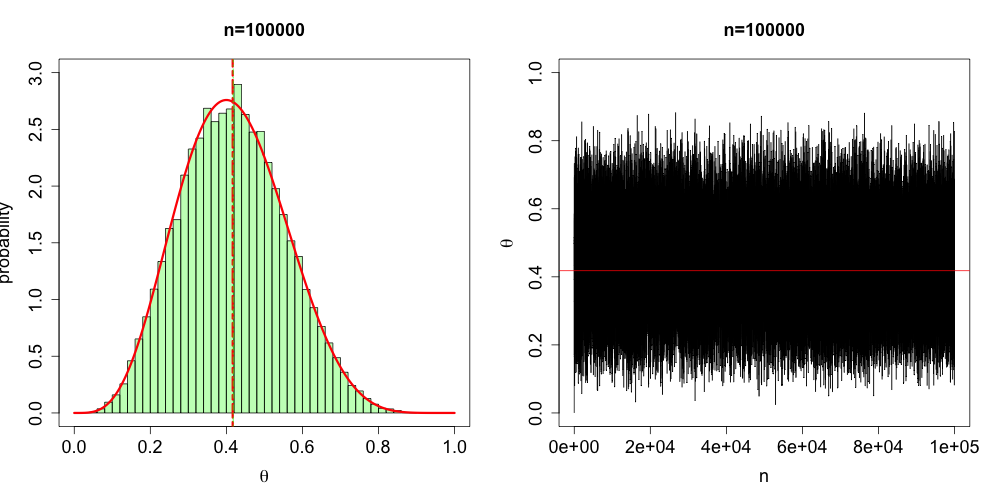
\includegraphics[width=0.7\textwidth]{mhexample2}
		\caption[Yksiulotteinen Metropolis--Hastings esimerkki]{Esimerkin \ref{MH-esim2} tulokset}
		\label{kuva2}
	\end{figure}

	Otetaan toisena esimerkkinä klassinen tapaus, jossa oletetaan, että havainnot ovat jakautuneet \textit{Bernoulli-jakauman} mukaan, 
	$y_i \sim \mathrm{Bernoulli}(\theta)$, 
	ja että priori on tasajakauma. Tällöin tiedetään, että analyyttinen posteriori on 
	\begin{equation*}
		p(\theta|y_i) = \mathrm{Beta}(\sum_{i=1}^{n} y_i+1, n - \sum_{i=1}^{n} y_i+1)
	\end{equation*}
	Valitaan hieman eksoottinen ehdotusjakauma esimerkin vuoksi:
	\begin{equation}
		J_n(\tn|\tnm) \sim \begin{cases}
			\mathrm{Unif}(\tnm,1) & \text{kun } \tnm<0.5 \\
			\mathrm{Unif}(0,\tnm) & \text{kun } \tnm\geq0.5
		\end{cases}
	\end{equation}
	Toisin kuin esimerkissä \ref{mh-esim1}, nyt ehdotusjakauma ei olekkaan symmetrinen.
	
	Oletetaan että, meillä on havainnot $(1,1,1,0,0,1,0,0,0,0)$ ja tarkastellaan sekä analyyttistä että MH-algoritmin tuottamaa jakaumaa ja niiden eroja.

	Kuvasta \ref{kuva2} nähdään esimerkin tulokset. Huomataan, että vaikka ehdotusjakauma on melko kummallinen, niin kuitenkin riittävän monella iteraatiolla saavutetaan tasapainojakauma. Huomaa, että vasemmassa kuvaajassa on vihreällä simulaatio keskiarvo, ja punaisella analyyttinen keskiarvo, mutta nämä arvot ovat niin lähellä toisiaan, että viivat ovat päällekkäin.
\end{esim}

\subsection{Yhteys Gibbsin otanta-algoritmiin}

Kuten jo totesimme aiemmin, Gibbsin otanta-algoritmin voi esittää Metropolis-Hastings algoritmin erityis tilanteena, jossa hyväksymistodennäköisyys on 1. \cite{gelman_andrew_bayesian_nodate}

\begin{lause}
	Gibbsin otanta-algoritmi on erityistapaus Metropolis-hastings algoritmista.
\end{lause}

\begin{proof}
	Määritellään MH-algoritmin iteraatio $n$ niin, että  se sisältää $d$ askelta, ja jossa iteraation $n$ askel $j$ kuvaa parametriosavektorin $\theta_j$ päivitystä ehdollistettuna kaikilla muilla parametrin $\theta$:n elementeillä. Tällöin ehdotusjakauma $J_{j,n}$ iteraation $n$ askeleessa $j$, voidaan määrittää siten, että se ehdottaa vain tiloja, jotka muuttaa vain parametria $\theta_j$. Eli:
	\begin{equation}
		J_{j,n}^{Gibbs}(\theta^*|\tnm)=\begin{cases}
			p(\theta^*_j|\tnm_{-j}) \qq{kun} \theta^*_{-j}=\tnm_{-j} \\
			0 \qq{muulloin}
		\end{cases}
	\end{equation}
	Nyt voidaan kirjoittaa suhde $r$ iteraation $n$ $j$:nen askeleen kohdalla muotoon
	\begin{equation}
		\begin{split}
			r &= \frac{p(\theta^*)/J_{j,n}^{Gibbs}(\theta^*|\tnm)}
			{p(\tnm)/J_{j,n}^{Gibbs}(\tnm|\theta^*)} \\
			&= \frac{p(\theta^*)/p(\theta^*_j|\tnm_{-j})}
			{p(\tnm)/p(\tnm_{j}|\tnm_{-j})} \\
			&= \frac{p(\tnm_{-j})}{p(\tnm_{-j})} \\
			&= 1
		\end{split}
	\end{equation}
	Eli määrittelemällä MH-algoritmille siirtymäjakauma sillä tavalla, että se vastaa Gibbsin otanta-algoritmia, siirtymän hyväksymistodennäköisyydeksi tulee 1.
	
\end{proof}

\subsection{Ehdotusjakauman valinnasta}

Kummassakin kappaleen \ref{Metropolis--Hastings algoritmi} esimerkissä valitsimme ehdotusjakauman melko satunnaisesti. Varsinkin esimerkissä \ref{MH-esim2} se on erittäin epätavallinen, mistä syystä hyvän approksimaation saavuttaminen vie todella monta iteraatiota. Yleensä jos haluamme oikeasti tehokkaasti ja ekonomisesti simuloida jakaumia esitetyllä algoritmilla, haluamme valita ehdotusjakauman jollakin järkevällä, systemaattisella tavalla, joka minimoisi tarvittavien iteraatioiden määrän.

Yleisesti ottaen hyvällä ehdotusjakaumalla on muutama ominaisuus\cite[s.~280]{gelman_andrew_bayesian_nodate}
\begin{enumerate}
	\item Kaikilla $\theta$:n arvoilla on helppo arpoa arvo $J(\theta'|\theta)$
	\item Suhde $r$ on helppo laskea
	\item Siirtymät ovat tarpeaksi pitkiä. Muuten Markovin ketju etenee liian hitaasti ja hyvän estimaatin saaminen kestää liian pitkään.
	\item Siirtymiä ei hylätä liian usein. Muuten Markovin ketju ei etene vaan seisoo paikallaan.
\end{enumerate}
Lisäksi simulointia voidaan nopeuttaa mm. käyttämällä adaptiivista ehdotusjakaumaa, jossa ehdotusjakaumaa muunnellaan riippuen ketjun liikkeistä. \cite[s.~295]{gelman_andrew_bayesian_nodate}
















